\let\negmedspace\undefined
\let\negthickspace\undefined
\documentclass[journal]{IEEEtran}
\usepackage[a5paper, margin=10mm, onecolumn]{geometry}
%\usepackage{lmodern} % Ensure lmodern is loaded for pdflatex
\usepackage{tfrupee} % Include tfrupee package

\setlength{\headheight}{1cm} % Set the height of the header box
\setlength{\headsep}{0mm}     % Set the distance between the header box and the top of the text

\usepackage{gvv-book}
\usepackage{gvv}
\usepackage{cite}
\usepackage{amsmath,amssymb,amsfonts,amsthm}
\usepackage{algorithmic}
\usepackage{graphicx}
\usepackage{textcomp}
\usepackage{xcolor}
\usepackage{txfonts}
\usepackage{listings}
\usepackage{enumitem}
\usepackage{mathtools}
\usepackage{gensymb}
\usepackage{comment}
\usepackage[breaklinks=true]{hyperref}
\usepackage{tkz-euclide} 
\usepackage{listings}
% \usepackage{gvv}                                        
\def\inputGnumericTable{}                                 
\usepackage[latin1]{inputenc}                                
\usepackage{color}                                            
\usepackage{array}                                            
\usepackage{longtable}                                       
\usepackage{calc}                                             
\usepackage{multirow}                                         
\usepackage{hhline}                                           
\usepackage{ifthen}                                           
\usepackage{lscape}
\begin{document}

\bibliographystyle{IEEEtran}
\vspace{3cm}

\title{5.8.4}
\author{EE25BTECH11006 - ADUDOTLA SRIVIDYA}
% \maketitle
% \newpage
% \bigskip
{\let\newpage\relax\maketitle}

\renewcommand{\thefigure}{\theenumi}
\renewcommand{\thetable}{\theenumi}
\setlength{\intextsep}{10pt} % Space between text and floats
\textbf{Question}:\\
 Half the perimeter of a rectangular garden, whose length is $4m$, more than its width,
 is $36m$. Find the dimensions of the garden.
 
\textbf{Solution}:\\
 
\begin{align}
    perimeter = 2(l+b)
\end{align}

\begin{align}
    \implies l+b = 18
\end{align}

given,
\begin{align}
    l-b = 4
\end{align}

\begin{align}
    \myvec{1&1\\1&-1}\myvec{l\\b} = \myvec{18\\4}
\end{align}

\begin{align}
    \augvec{2}{1}{1&1&18\\1&-1&4}
\end{align}
\begin{align}
    R_2 \to R_2-R_1 \implies \augvec{2}{1}{1&1&18\\0&-2&-14}
\end{align}
\begin{align}
    R_2 \to -1/2 R_2 \implies \augvec{2}{1}{1&1&18\\0&1&7}
\end{align}
\begin{align}
    R_1 \to R_1-R_2 \implies \augvec{2}{1}{1&0&11\\0&1&7}
\end{align}
\begin{align}
    \implies \myvec{l\\b} = \myvec{11\\7}
\end{align}
Therefore,
\begin{align}
    l=11 \ \ \ \ \
    b=7
\end{align}

\begin{figure}[H]
\begin{center}
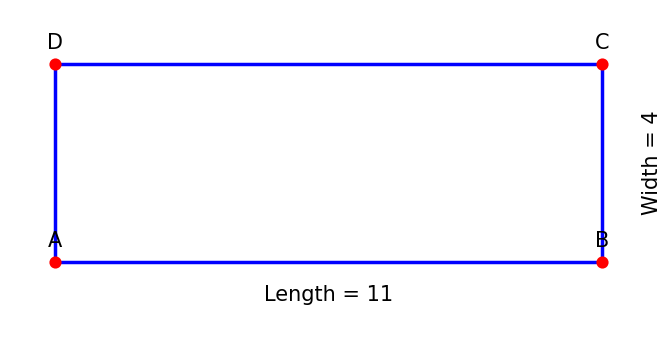
\includegraphics[width=0.7\columnwidth]{figs/fig.png}
\end{center}
\label{fig:Fig1}
\end{figure}

\end{document}